\documentclass[11pt,a4paper]{report}

% Packages
\usepackage[utf8]{inputenc}
\usepackage[T1]{fontenc}
\usepackage{geometry}
\usepackage{graphicx}
\usepackage{xcolor}
\usepackage{listings}
\usepackage{hyperref}
\usepackage{booktabs}
\usepackage{longtable}
\usepackage{fancyhdr}
\usepackage{titlesec}
\usepackage{tocloft}
\usepackage{enumitem}
\usepackage{tikz}
\usepackage{float}
\usepackage{caption}
\usepackage{subcaption}
\usepackage{multirow}
\usepackage{array}
\usepackage{tabularx}
\usepackage{fancyvrb}
\usepackage{mdframed}
\usepackage{tcolorbox}

% Page geometry
\geometry{
    top=1in,
    bottom=1in,
    left=1in,
    right=1in
}

% Colors
\definecolor{pittblue}{RGB}{0, 53, 148}
\definecolor{pittgold}{RGB}{255, 184, 28}
\definecolor{codegreen}{RGB}{0, 128, 0}
\definecolor{codegray}{RGB}{128, 128, 128}
\definecolor{codepurple}{RGB}{128, 0, 128}
\definecolor{backcolour}{RGB}{245, 245, 245}
\definecolor{terminalblack}{RGB}{30, 30, 30}
\definecolor{terminalgreen}{RGB}{0, 255, 0}

% Hyperref setup
\hypersetup{
    colorlinks=true,
    linkcolor=pittblue,
    filecolor=pittblue,
    urlcolor=pittblue,
    citecolor=pittblue,
    pdftitle={URC Complete Documentation},
    pdfauthor={University of Pittsburgh Robotics Club},
}

% Code listing style
\lstdefinestyle{codestyle}{
    backgroundcolor=\color{backcolour},
    commentstyle=\color{codegreen},
    keywordstyle=\color{pittblue}\bfseries,
    numberstyle=\tiny\color{codegray},
    stringstyle=\color{codepurple},
    basicstyle=\ttfamily\footnotesize,
    breakatwhitespace=false,
    breaklines=true,
    captionpos=b,
    keepspaces=true,
    numbers=left,
    numbersep=5pt,
    showspaces=false,
    showstringspaces=false,
    showtabs=false,
    tabsize=2,
    frame=single,
    rulecolor=\color{pittblue},
}

\lstdefinestyle{terminal}{
    backgroundcolor=\color{terminalblack},
    basicstyle=\ttfamily\footnotesize\color{white},
    breaklines=true,
    frame=single,
    rulecolor=\color{codegray},
}

\lstset{style=codestyle}

% Custom box for important notes
\tcbuselibrary{skins,breakable}
\newtcolorbox{importantbox}{
    colback=pittgold!10,
    colframe=pittgold,
    title=Important,
    fonttitle=\bfseries,
    breakable,
}

\newtcolorbox{warningbox}{
    colback=red!10,
    colframe=red!70,
    title=Warning,
    fonttitle=\bfseries,
    breakable,
}

\newtcolorbox{tipbox}{
    colback=green!10,
    colframe=green!50!black,
    title=Tip,
    fonttitle=\bfseries,
    breakable,
}

% Header and footer
\pagestyle{fancy}
\fancyhf{}
\fancyhead[L]{\leftmark}
\fancyhead[R]{URC Documentation}
\fancyfoot[C]{\thepage}
\renewcommand{\headrulewidth}{0.4pt}
\renewcommand{\footrulewidth}{0.4pt}

% Title formatting
\titleformat{\chapter}[display]
    {\normalfont\huge\bfseries\color{pittblue}}
    {\chaptertitlename\ \thechapter}{20pt}{\Huge}

\titleformat{\section}
    {\normalfont\Large\bfseries\color{pittblue}}
    {\thesection}{1em}{}

\titleformat{\subsection}
    {\normalfont\large\bfseries\color{pittblue!80}}
    {\thesubsection}{1em}{}

% Document info
\title{
    \vspace{-2cm}
    \includegraphics[width=0.3\textwidth]{example-image}\\ % Replace with actual logo
    \vspace{1cm}
    {\color{pittblue}\Huge\bfseries University Rover Challenge}\\
    \vspace{0.5cm}
    {\color{pittblue!70}\LARGE Complete Technical Documentation}\\
    \vspace{0.5cm}
    {\large\color{pittgold} \& Startup Guide}
}
\author{
    \textbf{University of Pittsburgh Robotics Club}\\
    \vspace{0.5cm}
    \small ROS 2 Humble $\bullet$ NVIDIA Jetson Nano $\bullet$ Docker
}
\date{Version 2.0 --- January 2026}

\begin{document}

% Title page
\maketitle
\thispagestyle{empty}

\vfill
\begin{center}
\begin{tabular}{ll}
\textbf{Platform:} & ROS 2 Humble Hawksbill \\
\textbf{Hardware:} & NVIDIA Jetson Nano, Arduino \\
\textbf{Deployment:} & Docker Containers \\
\textbf{GUI:} & PyQt5 \\
\end{tabular}
\end{center}

\newpage

% Table of Contents
\tableofcontents
\newpage

% List of Figures and Tables
\listoffigures
\listoftables
\newpage

%=============================================================================
\chapter{Project Overview}
%=============================================================================

\section{Introduction}

This document provides comprehensive technical documentation for the University of Pittsburgh Robotics Club's University Rover Challenge (URC) rover system. The system integrates advanced robotics technologies including:

\begin{itemize}
    \item \textbf{6-wheel differential drive system} with GoBilda motors
    \item \textbf{Multi-sensor fusion} including GPS, IMU, ultrasonic sensors, and cameras
    \item \textbf{ROS 2 Humble} for distributed robot communication
    \item \textbf{Docker containerization} for reproducible deployments
    \item \textbf{PyQt5 GUI system} for teleoperation and monitoring
\end{itemize}

\section{Competition Tasks}

The University Rover Challenge consists of multiple mission types:

\begin{table}[H]
\centering
\caption{URC Competition Tasks}
\begin{tabular}{@{}lp{10cm}@{}}
\toprule
\textbf{Task} & \textbf{Description} \\
\midrule
Autonomous Navigation & GPS-guided traversal of challenging Martian-analog terrain \\
Equipment Servicing & Precise manipulation tasks using robotic arm \\
Extreme Delivery & Package delivery in harsh environmental conditions \\
Science Operations & Sample collection and in-field analysis \\
Teleoperation & Manual control for complex scenarios \\
\bottomrule
\end{tabular}
\end{table}

\section{Key Specifications}

\begin{table}[H]
\centering
\caption{Rover System Specifications}
\begin{tabular}{@{}ll@{}}
\toprule
\textbf{Metric} & \textbf{Value} \\
\midrule
Navigation Accuracy & $\pm$2m GPS positioning \\
Video Latency & $<$200ms streaming \\
Control Response & $<$50ms command execution \\
Battery Life & 4+ hours autonomous operation \\
Operating Range & 1km+ radio communication \\
Motor Control & 6 GoBilda motors (0--255 PWM) \\
Camera Frame Rate & 30 Hz \\
IMU Update Rate & 10 Hz \\
Serial Baud Rate & 115200 bps \\
\bottomrule
\end{tabular}
\end{table}

%=============================================================================
\chapter{System Architecture}
%=============================================================================

\section{High-Level Architecture}

The rover system uses a \textbf{dual-container architecture} for optimal performance and separation of concerns.

\begin{figure}[H]
\centering
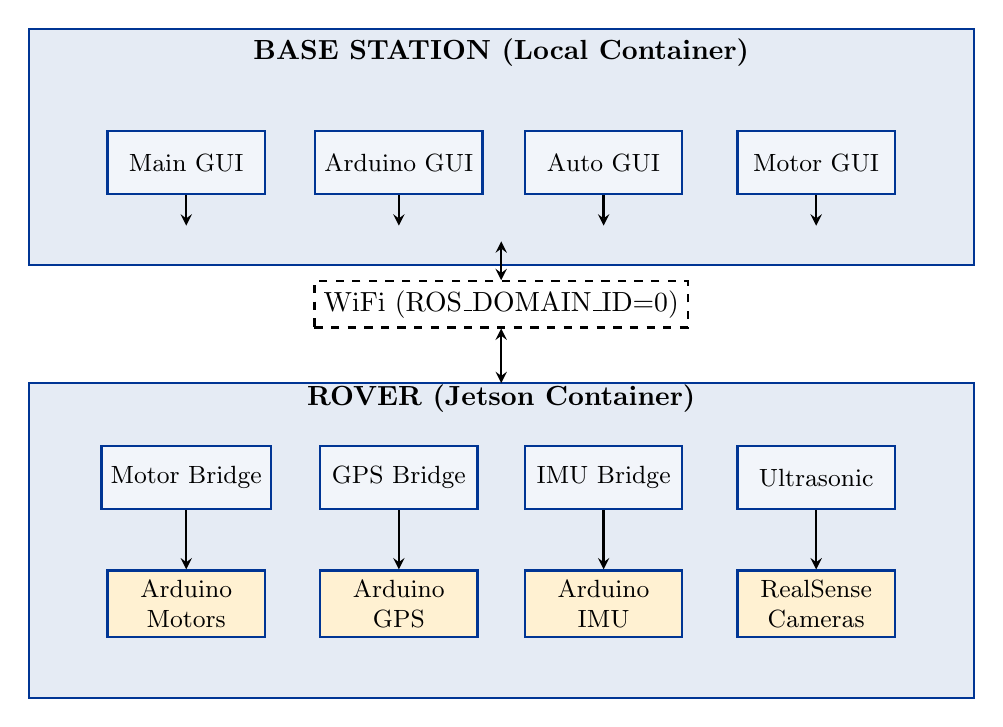
\begin{tikzpicture}[
    node distance=1.5cm,
    box/.style={rectangle, draw=pittblue, thick, minimum width=3cm, minimum height=1cm, align=center, fill=pittblue!10},
    smallbox/.style={rectangle, draw=pittblue, thick, minimum width=2cm, minimum height=0.8cm, align=center, fill=pittblue!5, font=\small},
    arrow/.style={->, thick, >=stealth}
]
    % Base Station
    \node[box, minimum width=12cm, minimum height=3cm] (base) at (0, 4) {};
    \node at (0, 5.2) {\textbf{BASE STATION (Local Container)}};

    \node[smallbox] (gui1) at (-4, 3.8) {Main GUI};
    \node[smallbox] (gui2) at (-1.3, 3.8) {Arduino GUI};
    \node[smallbox] (gui3) at (1.3, 3.8) {Auto GUI};
    \node[smallbox] (gui4) at (4, 3.8) {Motor GUI};

    % WiFi Connection
    \node[draw, dashed, thick, minimum width=3cm] (wifi) at (0, 2) {WiFi (ROS\_DOMAIN\_ID=0)};

    % Rover
    \node[box, minimum width=12cm, minimum height=4cm] (rover) at (0, -1) {};
    \node at (0, 0.8) {\textbf{ROVER (Jetson Container)}};

    \node[smallbox] (motor) at (-4, -0.2) {Motor Bridge};
    \node[smallbox] (gps) at (-1.3, -0.2) {GPS Bridge};
    \node[smallbox] (imu) at (1.3, -0.2) {IMU Bridge};
    \node[smallbox] (ultra) at (4, -0.2) {Ultrasonic};

    \node[smallbox, fill=pittgold!20] (arduino1) at (-4, -1.8) {Arduino\\Motors};
    \node[smallbox, fill=pittgold!20] (arduino2) at (-1.3, -1.8) {Arduino\\GPS};
    \node[smallbox, fill=pittgold!20] (arduino3) at (1.3, -1.8) {Arduino\\IMU};
    \node[smallbox, fill=pittgold!20] (camera) at (4, -1.8) {RealSense\\Cameras};

    % Arrows
    \draw[arrow] (gui1) -- ++(0, -0.8);
    \draw[arrow] (gui2) -- ++(0, -0.8);
    \draw[arrow] (gui3) -- ++(0, -0.8);
    \draw[arrow] (gui4) -- ++(0, -0.8);

    \draw[arrow, <->] (0, 2.8) -- (wifi);
    \draw[arrow, <->] (wifi) -- (0, 1);

    \draw[arrow] (motor) -- (arduino1);
    \draw[arrow] (gps) -- (arduino2);
    \draw[arrow] (imu) -- (arduino3);
    \draw[arrow] (ultra) -- (camera);

\end{tikzpicture}
\caption{System Architecture Overview}
\end{figure}

\section{Dual-Container Architecture}

\begin{table}[H]
\centering
\caption{Container Responsibilities}
\begin{tabular}{@{}llp{7cm}@{}}
\toprule
\textbf{Container} & \textbf{Location} & \textbf{Purpose} \\
\midrule
Jetson Container & On-board rover & Hardware bridges, sensor acquisition, motor control, camera feeds \\
Local Container & Base station & GUI interfaces, visualization, high-level control, debugging \\
\bottomrule
\end{tabular}
\end{table}

\begin{tipbox}
The dual-container architecture saves Jetson processing power for real-time control while enabling easier debugging with local GUI applications. ROS 2 communication works seamlessly over WiFi.
\end{tipbox}

\section{Communication Flow}

\begin{figure}[H]
\centering
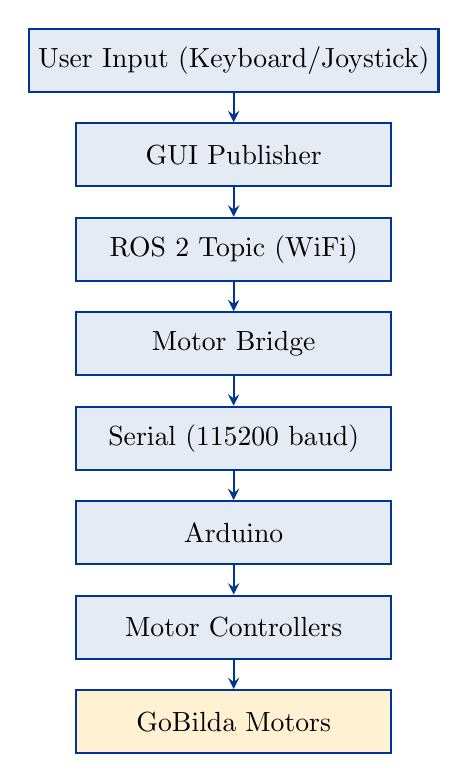
\begin{tikzpicture}[
    node distance=1.2cm,
    box/.style={rectangle, draw=pittblue, thick, minimum width=4cm, minimum height=0.8cm, align=center, fill=pittblue!10},
    arrow/.style={->, thick, >=stealth, pittblue}
]
    \node[box] (input) {User Input (Keyboard/Joystick)};
    \node[box, below of=input] (pub) {GUI Publisher};
    \node[box, below of=pub] (topic) {ROS 2 Topic (WiFi)};
    \node[box, below of=topic] (bridge) {Motor Bridge};
    \node[box, below of=bridge] (serial) {Serial (115200 baud)};
    \node[box, below of=serial] (arduino) {Arduino};
    \node[box, below of=arduino] (controller) {Motor Controllers};
    \node[box, below of=controller, fill=pittgold!20] (motors) {GoBilda Motors};

    \draw[arrow] (input) -- (pub);
    \draw[arrow] (pub) -- (topic);
    \draw[arrow] (topic) -- (bridge);
    \draw[arrow] (bridge) -- (serial);
    \draw[arrow] (serial) -- (arduino);
    \draw[arrow] (arduino) -- (controller);
    \draw[arrow] (controller) -- (motors);
\end{tikzpicture}
\caption{Motor Control Communication Flow}
\end{figure}

%=============================================================================
\chapter{Directory Structure}
%=============================================================================

\section{Project Layout}

The project follows a modular organization:

\begin{lstlisting}[language=bash, caption={Project Directory Structure}]
URC/
|-- docker/                    # Docker configuration
|   |-- jetson/               # On-board Jetson container
|   |   |-- Dockerfile
|   |   |-- docker-compose.yml
|   |   |-- start.sh
|   |   |-- supervisord.conf
|   |   +-- setup.py
|   |-- jetson_local/         # Alternative Jetson setup
|   +-- local/                # Base station container
|       |-- Dockerfile
|       |-- docker-compose.yml
|       |-- start_mac.sh
|       |-- start_linux.sh
|       +-- sim-launch.sh
|
|-- ros_bridge/               # ROS 2 hardware bridges
|   |-- arduino_bridge_base/  # Base class for bridges
|   |-- motor_bridge/         # Motor control system
|   |-- motor_subscriber/     # Legacy motor control
|   |-- gps_bridge/           # GPS sensor bridge
|   |-- imu_bridge/           # IMU sensor bridge
|   +-- ultrasonic_bridge/    # Ultrasonic sensor bridge
|
|-- guis/                     # PyQt5 GUI applications
|   |-- gen_gui.py            # Main control dashboard
|   |-- arduino_gui.py        # Hardware control interface
|   |-- auto_gui.py           # Autonomous navigation
|   |-- json_motorGUI.py      # Motor/Arm keyboard control
|   |-- publishers/           # ROS 2 publisher classes
|   |-- subscribers/          # ROS 2 subscriber classes
|   +-- camera/               # Camera utilities
|
|-- simulation/               # Gazebo simulation
|   +-- colcon_ws/            # ROS 2 workspace
|
|-- README.md
|-- CONTRIBUTING.md
+-- Makefile
\end{lstlisting}

\section{Key Directories}

\subsection{Docker Configuration}

\begin{itemize}
    \item \texttt{docker/jetson/} --- On-board rover container with NVIDIA runtime support
    \item \texttt{docker/local/} --- Base station container with X11 forwarding for GUI
    \item \texttt{docker/jetson\_local/} --- Alternative hybrid setup
\end{itemize}

\subsection{ROS Bridge}

\begin{itemize}
    \item \texttt{arduino\_bridge\_base/} --- Base class providing serial communication (248 lines)
    \item \texttt{motor\_bridge/} --- Unified motor control with multiple input sources
    \item \texttt{gps\_bridge/} --- NMEA sentence parsing and publishing
    \item \texttt{imu\_bridge/} --- BNO055 9-axis IMU integration
    \item \texttt{ultrasonic\_bridge/} --- Multi-sensor distance measurement
\end{itemize}

\subsection{GUI System}

\begin{itemize}
    \item \texttt{gen\_gui.py} --- Main dashboard (623 lines) with camera feeds and sensor data
    \item \texttt{arduino\_gui.py} --- Joystick-style motor control (617 lines)
    \item \texttt{json\_motorGUI.py} --- Keyboard hotkey control (292 lines)
    \item \texttt{publishers/} --- MotorPublisher, TwistPublisher classes
    \item \texttt{subscribers/} --- IMUSubscriber, GPSSubscriber, data parsers
\end{itemize}

%=============================================================================
\chapter{Hardware Requirements}
%=============================================================================

\section{On-Board Computer}

\begin{table}[H]
\centering
\caption{Jetson Nano Specifications}
\begin{tabular}{@{}ll@{}}
\toprule
\textbf{Component} & \textbf{Specification} \\
\midrule
Computer & NVIDIA Jetson Nano (4GB) \\
Storage & 64GB+ SD Card or NVMe SSD \\
Power & 5V 4A barrel jack \\
Cooling & Active fan (recommended) \\
\bottomrule
\end{tabular}
\end{table}

\section{Motor System}

\begin{table}[H]
\centering
\caption{Motor System Specifications}
\begin{tabular}{@{}ll@{}}
\toprule
\textbf{Component} & \textbf{Specification} \\
\midrule
Motors & 6x GoBilda motors \\
Motor Controllers & 3x dual H-bridge controllers \\
Arduino & Arduino Mega 2560 (recommended) \\
PWM Range & 0--255 \\
Wheel Base & 0.7384 meters \\
Max Speed & 1.0 m/s \\
\bottomrule
\end{tabular}
\end{table}

\subsection{Pin Configuration}

\begin{table}[H]
\centering
\caption{Arduino Motor Pin Configuration}
\begin{tabular}{@{}lccl@{}}
\toprule
\textbf{Motor} & \textbf{PWM Pin} & \textbf{Direction Pin} & \textbf{Side} \\
\midrule
Front Left & 2 & 53 & Left \\
Middle Left & 4 & 51 & Left \\
Back Left & 6 & 49 & Left \\
Front Right & 3 & 52 & Right \\
Middle Right & 5 & 50 & Right \\
Back Right & 7 & 48 & Right \\
\bottomrule
\end{tabular}
\end{table}

\section{Sensors}

\begin{table}[H]
\centering
\caption{Sensor Configuration}
\begin{tabular}{@{}lllc@{}}
\toprule
\textbf{Sensor} & \textbf{Model} & \textbf{Connection} & \textbf{Rate} \\
\midrule
IMU & Adafruit BNO055 (9-axis) & Serial 115200 & 10 Hz \\
GPS & RTK GPS module & Serial 115200 & 1 Hz \\
Cameras & 2x Intel RealSense D435 & USB 3.0 & 30 Hz \\
Ultrasonic & 3x HC-SR04 & Arduino GPIO & 10 Hz \\
\bottomrule
\end{tabular}
\end{table}

\subsection{Ultrasonic Sensor Pins}

\begin{table}[H]
\centering
\caption{Ultrasonic Sensor Pin Configuration}
\begin{tabular}{@{}lcc@{}}
\toprule
\textbf{Sensor} & \textbf{Trigger Pin} & \textbf{Echo Pin} \\
\midrule
Sensor 1 & 8 & 9 \\
Sensor 2 & 50 & 51 \\
Sensor 3 & 48 & 49 \\
\bottomrule
\end{tabular}
\end{table}

\section{Serial Port Configuration}

\begin{table}[H]
\centering
\caption{Serial Port Assignments}
\begin{tabular}{@{}llll@{}}
\toprule
\textbf{Device} & \textbf{Port} & \textbf{Baud Rate} & \textbf{Notes} \\
\midrule
Motors & /dev/ttyACM1 & 115200 & Hardcoded in MotorBridge \\
GPS & /dev/ttyACM0 & 115200 & Configurable \\
IMU & Auto-detect & 115200 & Tries multiple ports \\
Ultrasonic & Arduino internal & 115200 & No separate port \\
\bottomrule
\end{tabular}
\end{table}

%=============================================================================
\chapter{Software Dependencies}
%=============================================================================

\section{System Requirements}

\begin{itemize}
    \item \textbf{Operating System:} Ubuntu 22.04 LTS
    \item \textbf{ROS Version:} ROS 2 Humble Hawksbill
    \item \textbf{Python:} 3.10+
    \item \textbf{Docker:} 20.10+
\end{itemize}

\section{Python Dependencies}

\begin{lstlisting}[language=bash, caption={Python Package Requirements}]
# Core ROS 2
rclpy
ros2cli

# Hardware Communication
pyserial>=3.5
pyrealsense2>=2.50.0

# GUI Framework
PyQt5>=5.15.0
PyQt5-sip

# Computer Vision
opencv-python>=4.5.0
numpy<2.0

# ROS 2 Message Bridges
cv_bridge
sensor_msgs
geometry_msgs
std_msgs
\end{lstlisting}

\section{System Packages (APT)}

\begin{lstlisting}[language=bash, caption={System Package Requirements}]
# Base development
python3-pip python3-pyqt5 python3-pyqt5.qtsvg

# Graphics libraries (for GUI)
libxcb-xinerama0 libxcb-cursor0 libxkbcommon-x11-0
libgl1-mesa-glx libgl1-mesa-dri mesa-utils x11-apps

# ROS 2 Humble
ros-humble-desktop ros-dev-tools
ros-humble-teleop-twist-keyboard ros-humble-joy

# Intel RealSense
librealsense2-utils librealsense2-dev
ros-humble-librealsense2-* ros-humble-realsense2-*
\end{lstlisting}

\section{Arduino Libraries}

\begin{itemize}
    \item \texttt{Adafruit\_Sensor} --- Unified sensor abstraction layer
    \item \texttt{Adafruit\_BNO055} --- 9-axis IMU driver library
\end{itemize}

%=============================================================================
\chapter{Docker Configuration}
%=============================================================================

\section{Jetson Container}

\subsection{Overview}

The Jetson container runs on-board the rover and manages all hardware interfaces.

\begin{lstlisting}[language=bash, caption={Build and Start Jetson Container}]
cd docker/jetson
sudo docker build -t urc_jetson .
sudo docker-compose up -d
\end{lstlisting}

\subsection{Key Features}

\begin{itemize}
    \item NVIDIA GPU support (\texttt{runtime: nvidia})
    \item Privileged mode for device access
    \item Host network mode for ROS 2 communication
    \item Supervisor process management
\end{itemize}

\subsection{Device Mappings}

\begin{lstlisting}[language=yaml, caption={Docker Compose Device Configuration}]
devices:
  - /dev:/dev                    # All devices
  - /dev/bus/usb:/dev/bus/usb    # USB devices
  - /dev/video0:/dev/video0      # Camera 1
  - /dev/video1:/dev/video1      # Camera 2
\end{lstlisting}

\subsection{Environment Variables}

\begin{lstlisting}[language=yaml, caption={Jetson Environment Variables}]
environment:
  - ROS_DOMAIN_ID=0
  - ROS_LOCALHOST_ONLY=0
  - NVIDIA_DRIVER_CAPABILITIES=all
  - NVIDIA_VISIBLE_DEVICES=all
\end{lstlisting}

\subsection{Supervised Processes}

\begin{table}[H]
\centering
\caption{Supervisor Managed Processes}
\begin{tabular}{@{}llc@{}}
\toprule
\textbf{Process} & \textbf{Description} & \textbf{Auto-restart} \\
\midrule
setup & RealSense camera initialization & Yes \\
gps\_bridge & GPS data publisher & Yes \\
motor\_bridge & Motor command handler & Yes \\
ultrasonic\_bridge & Ultrasonic sensor publisher & Yes \\
\bottomrule
\end{tabular}
\end{table}

\section{Local Container (Base Station)}

\subsection{macOS Setup}

\begin{lstlisting}[language=bash, caption={macOS Container Startup}]
# Prerequisite: Install XQuartz and enable network clients
# System Preferences > Security > Allow connections

cd docker/local
chmod +x start_mac.sh
./start_mac.sh
\end{lstlisting}

\subsection{Linux Setup}

\begin{lstlisting}[language=bash, caption={Linux Container Startup}]
cd docker/local
chmod +x start_linux.sh
./start_linux.sh
\end{lstlisting}

\subsection{Local Environment Variables}

\begin{lstlisting}[language=yaml, caption={Local Container Environment}]
environment:
  - ROS_DOMAIN_ID=0
  - ROS_LOCALHOST_ONLY=0
  - QT_X11_NO_MITSHM=1
  - DISPLAY=${DISPLAY}
\end{lstlisting}

\section{Simulation Container}

\begin{lstlisting}[language=bash, caption={Simulation Startup}]
cd docker/local
./sim-launch.sh

# Launch simulation
ros2 launch my_robot_description display.launch.py use_sim_time:=true
\end{lstlisting}

%=============================================================================
\chapter{Quick Start Guide}
%=============================================================================

\section{Prerequisites}

\subsection{Install Docker}

\begin{lstlisting}[language=bash, caption={Docker Installation}]
# Linux
curl -fsSL https://get.docker.com -o get-docker.sh
sudo sh get-docker.sh

# macOS
brew install --cask docker
\end{lstlisting}

\subsection{Clone Repository}

\begin{lstlisting}[language=bash, caption={Clone Repository}]
git clone https://github.com/pitt-robotics/URC.git
cd URC
\end{lstlisting}

\subsection{Connect Hardware}

\begin{enumerate}
    \item Connect Arduino to USB port
    \item Connect RealSense cameras to USB 3.0 ports
    \item Power on motor controllers
    \item Verify serial ports: \texttt{ls /dev/ttyACM*}
\end{enumerate}

\section{Option A: Full System Startup}

\begin{importantbox}
This option requires both the rover (Jetson) and base station (local machine) to be on the same WiFi network.
\end{importantbox}

\subsection{Step 1: Start Jetson Container (on rover)}

\begin{lstlisting}[language=bash]
cd docker/jetson
sudo ./start.sh
\end{lstlisting}

\subsection{Step 2: Start Local Container (on base station)}

\begin{lstlisting}[language=bash]
# macOS
cd docker/local
./start_mac.sh

# Linux
cd docker/local
./start_linux.sh
\end{lstlisting}

\subsection{Step 3: Launch GUI}

\begin{lstlisting}[language=bash]
# Inside local container
source /opt/ros/humble/local_setup.bash
cd /app
python3 -m guis.gen_gui
\end{lstlisting}

\section{Option B: Simulation Only}

\begin{lstlisting}[language=bash]
cd docker/local
./sim-launch.sh

# In another terminal (inside container)
ros2 launch my_robot_description display.launch.py use_sim_time:=true
\end{lstlisting}

\section{Option C: Development Mode}

\begin{lstlisting}[language=bash]
# Start local container
cd docker/local
./start_linux.sh

# Inside container
source /opt/ros/humble/local_setup.bash
cd /app

# Run individual components
python3 ros_bridge/motor_bridge/launch_motor_bridge.py
python3 -m guis.arduino_gui
\end{lstlisting}

%=============================================================================
\chapter{Detailed Startup Procedures}
%=============================================================================

\section{Jetson On-Board Startup}

\begin{lstlisting}[language=bash, caption={Complete Jetson Startup Procedure}]
# 1. SSH into Jetson
ssh nvidia@<jetson-ip>

# 2. Navigate to project
cd /path/to/URC

# 3. Build and start container (first time)
cd docker/jetson
sudo docker build -t urc_jetson .
sudo docker-compose up -d

# 4. Verify container is running
sudo docker ps

# 5. Check supervised processes
sudo docker exec -it pitt_urc_jetson supervisorctl status

# Expected output:
# gps_bridge          RUNNING   pid 123, uptime 0:01:00
# motor_bridge        RUNNING   pid 124, uptime 0:01:00
# setup               RUNNING   pid 125, uptime 0:01:00
# ultrasonic_bridge   RUNNING   pid 126, uptime 0:01:00

# 6. View logs
sudo docker exec -it pitt_urc_jetson tail -f /app/motor_bridge.log
\end{lstlisting}

\section{Base Station Startup}

\subsection{macOS Procedure}

\begin{lstlisting}[language=bash, caption={macOS Base Station Startup}]
# 1. Start XQuartz
open -a XQuartz

# 2. Enable network clients (if not done)
# XQuartz > Preferences > Security > Allow connections

# 3. Navigate to project
cd /path/to/URC/docker/local

# 4. Start container
./start_mac.sh

# 5. Source ROS 2
source /opt/ros/humble/local_setup.bash

# 6. Launch main GUI
cd /app
python3 -m guis.gen_gui
\end{lstlisting}

\subsection{Linux Procedure}

\begin{lstlisting}[language=bash, caption={Linux Base Station Startup}]
# 1. Navigate to project
cd /path/to/URC/docker/local

# 2. Start container
./start_linux.sh

# 3. Source ROS 2
source /opt/ros/humble/local_setup.bash

# 4. Launch main GUI
cd /app
python3 -m guis.gen_gui
\end{lstlisting}

\section{Verification Steps}

\subsection{Check ROS 2 Connectivity}

\begin{lstlisting}[language=bash, caption={ROS 2 Verification Commands}]
# List all active nodes
ros2 node list

# Expected:
# /motor_bridge
# /gps_bridge
# /imu_bridge
# /ultrasonic_bridge

# List all topics
ros2 topic list

# Expected:
# /cmd_vel
# /motor_control_input
# /drive_data
# /gps_data
# /imu_data
# /ultrasonic_data
# /camera/gray/image_raw
# /camera/depth/image_raw
\end{lstlisting}

\subsection{Test Motor Commands}

\begin{warningbox}
Be careful when testing motor commands! Ensure the rover is in a safe position before sending movement commands.
\end{warningbox}

\begin{lstlisting}[language=bash, caption={Motor Command Testing}]
# Send stop command
ros2 topic pub --once /motor_control_input std_msgs/String \
    "data: '0,0,0,0,0,0'"

# Send forward command (be careful!)
ros2 topic pub --once /motor_control_input std_msgs/String \
    "data: '100,0,0,0,0,0'"
\end{lstlisting}

\subsection{Monitor Sensor Data}

\begin{lstlisting}[language=bash, caption={Sensor Data Monitoring}]
# IMU data
ros2 topic echo /imu_data

# GPS data
ros2 topic echo /gps_data

# Ultrasonic data
ros2 topic echo /ultrasonic_data
\end{lstlisting}

%=============================================================================
\chapter{ROS 2 Architecture}
%=============================================================================

\section{Node Overview}

\begin{table}[H]
\centering
\caption{ROS 2 Nodes}
\begin{tabular}{@{}llp{6cm}@{}}
\toprule
\textbf{Node} & \textbf{Package} & \textbf{Purpose} \\
\midrule
motor\_bridge & ros\_bridge & Motor command handling and feedback \\
gps\_bridge & ros\_bridge & GPS NMEA data publishing \\
imu\_bridge & ros\_bridge & IMU orientation data publishing \\
ultrasonic\_bridge & ros\_bridge & Distance measurement publishing \\
gray\_and\_depth\_publisher & guis.camera & Camera feed publishing \\
\bottomrule
\end{tabular}
\end{table}

\section{Topic Architecture}

\begin{figure}[H]
\centering
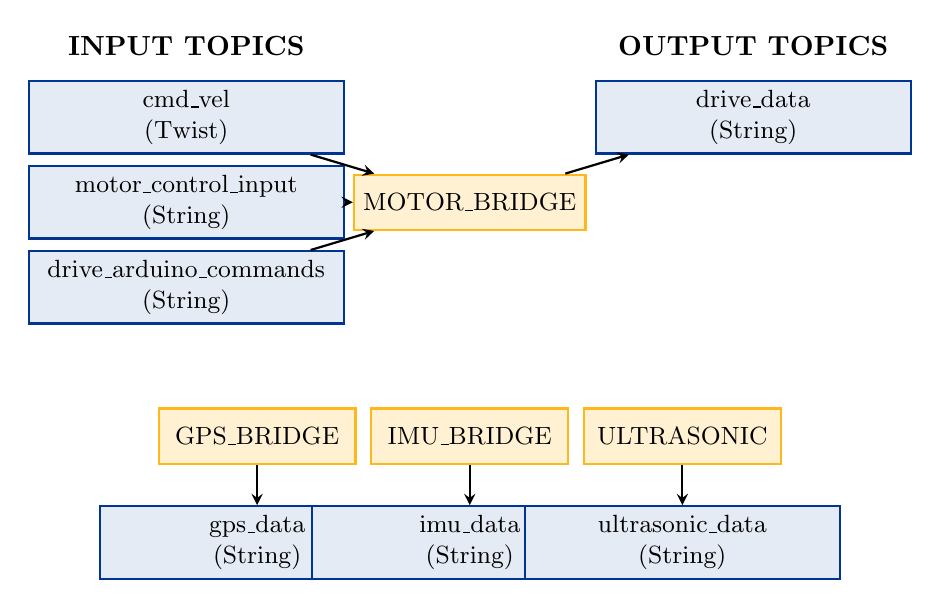
\begin{tikzpicture}[
    scale=0.9,
    node distance=0.8cm,
    topicbox/.style={rectangle, draw=pittblue, thick, minimum width=4cm, minimum height=0.7cm, align=center, fill=pittblue!10, font=\small},
    nodebox/.style={rectangle, draw=pittgold, thick, minimum width=2.5cm, minimum height=0.7cm, align=center, fill=pittgold!20, font=\small},
    arrow/.style={->, thick, >=stealth}
]
    % Input Topics
    \node at (-4, 5) {\textbf{INPUT TOPICS}};
    \node[topicbox] (cmdvel) at (-4, 4) {cmd\_vel\\(Twist)};
    \node[topicbox] (motor) at (-4, 2.8) {motor\_control\_input\\(String)};
    \node[topicbox] (legacy) at (-4, 1.6) {drive\_arduino\_commands\\(String)};

    % Motor Bridge
    \node[nodebox] (motorbridge) at (0, 2.8) {MOTOR\_BRIDGE};

    % Output Topics
    \node at (4, 5) {\textbf{OUTPUT TOPICS}};
    \node[topicbox] (drivedata) at (4, 4) {drive\_data\\(String)};

    % Sensor Bridges
    \node[nodebox] (gpsbridge) at (-3, -0.5) {GPS\_BRIDGE};
    \node[nodebox] (imubridge) at (0, -0.5) {IMU\_BRIDGE};
    \node[nodebox] (ultrabridge) at (3, -0.5) {ULTRASONIC};

    % Sensor Topics
    \node[topicbox] (gpsdata) at (-3, -2) {gps\_data\\(String)};
    \node[topicbox] (imudata) at (0, -2) {imu\_data\\(String)};
    \node[topicbox] (ultradata) at (3, -2) {ultrasonic\_data\\(String)};

    % Arrows
    \draw[arrow] (cmdvel) -- (motorbridge);
    \draw[arrow] (motor) -- (motorbridge);
    \draw[arrow] (legacy) -- (motorbridge);
    \draw[arrow] (motorbridge) -- (drivedata);

    \draw[arrow] (gpsbridge) -- (gpsdata);
    \draw[arrow] (imubridge) -- (imudata);
    \draw[arrow] (ultrabridge) -- (ultradata);

\end{tikzpicture}
\caption{ROS 2 Topic Architecture}
\end{figure}

\section{Message Formats}

\subsection{Motor Control Input (String)}

\begin{lstlisting}[caption={Motor Command Format}]
Format: "linear_x,linear_y,linear_z,angular_x,angular_y,angular_z"
Example: "100,0,0,0,0,50"  # Forward with slight right turn
\end{lstlisting}

\subsection{IMU Data (String)}

\begin{lstlisting}[caption={IMU Data Format}]
Format: "X: <value>\tY: <value>\tZ: <value>"
Example: "X: 0.123\tY: 0.456\tZ: 0.789"
\end{lstlisting}

\subsection{GPS Data (String)}

\begin{lstlisting}[caption={GPS NMEA Format}]
NMEA sentences:
$GNGLL,4024.12345,N,07952.12345,W,123456.00,A,A*6B
$GAGSV,3,1,12,01,45,123,38,02,67,234,42,...
\end{lstlisting}

\subsection{Ultrasonic Data (String)}

\begin{lstlisting}[caption={Ultrasonic Data Format}]
Format: "distance1_cm, distance2_cm, distance3_cm, "
Example: "45, 120, 88, "
\end{lstlisting}

\section{Bridge Class Hierarchy}

\begin{lstlisting}[language=python, caption={Bridge Class Structure}]
ArduinoBridgeBase(Node)           # Base class (248 lines)
    |-- MotorBridge               # Motor control
    |-- GPSBridge                 # GPS data
    |-- IMUBridge                 # IMU data
    +-- UltrasonicBridge          # Ultrasonic data
\end{lstlisting}

\textbf{Base Class Features:}
\begin{itemize}
    \item Serial port initialization (115200 baud)
    \item Generic ROS 2 topic subscription/publishing
    \item Timer-based Arduino reading (100ms default)
    \item Error handling and logging
    \item Automatic reconnection attempts
\end{itemize}

%=============================================================================
\chapter{Hardware Interfaces}
%=============================================================================

\section{Motor Control}

\subsection{Arduino Firmware}

\textbf{Location:} \texttt{ros\_bridge/motor\_subscriber/motor\_serial/motor\_serial.ino}

\begin{lstlisting}[language=C, caption={Motor Control Logic}]
// Simplified differential drive
left_speed = linear_x - angular_z;
right_speed = linear_x + angular_z;

// PWM mapping
pwm_left = map(left_speed, -100, 100, -255, 255);
pwm_right = map(right_speed, -100, 100, -255, 255);

// Direction Control
// HIGH = Forward
// LOW = Reverse
\end{lstlisting}

\section{IMU (BNO055)}

\textbf{Location:} \texttt{ros\_bridge/imu\_bridge/imu\_serial/imu\_serial.ino}

\begin{lstlisting}[language=C, caption={IMU Configuration}]
Adafruit_BNO055 bno = Adafruit_BNO055(55);
bno.setExtCrystalUse(true);  // External crystal for accuracy

// Output Format
Serial.print("X: "); Serial.print(event.orientation.x);
Serial.print("\tY: "); Serial.print(event.orientation.y);
Serial.print("\tZ: "); Serial.println(event.orientation.z);
\end{lstlisting}

\subsection{Data Processing}

\begin{lstlisting}[language=python, caption={IMU Data Parser}]
# IMUDataParser.py
import math

distance = math.sqrt(
    (x_cur - x_prev)**2 +
    (y_cur - y_prev)**2 +
    (z_cur - z_prev)**2
)
velocity = distance / time_delta
vertical_tilt = math.degrees(math.atan2(y_delta, z_delta))
horizontal_tilt = math.degrees(math.atan2(y_delta, x_delta))
\end{lstlisting}

\section{GPS}

\textbf{Location:} \texttt{ros\_bridge/gps\_bridge/gps/gps.ino}

\begin{table}[H]
\centering
\caption{NMEA Sentence Types}
\begin{tabular}{@{}ll@{}}
\toprule
\textbf{Type} & \textbf{Purpose} \\
\midrule
GNGLL & Geographic position (latitude/longitude) \\
GAGSV & GPS satellites in view + SNR \\
GBGSV & BeiDou satellites in view + SNR \\
\bottomrule
\end{tabular}
\end{table}

\section{Ultrasonic Sensors}

\textbf{Location:} \texttt{ros\_bridge/ultrasonic\_bridge/multiple\_untrasonic\_sensors/}

\begin{lstlisting}[language=C, caption={Ultrasonic Distance Calculation}]
duration = pulseIn(echoPin, HIGH);
distance_cm = (duration / 2) / 29.1;
\end{lstlisting}

\section{RealSense Cameras}

\textbf{Location:} \texttt{guis/camera/camera\_cv\_test.py}

\begin{lstlisting}[language=python, caption={RealSense Configuration}]
import pyrealsense2 as rs

# Color stream
config.enable_stream(rs.stream.color, 640, 480, rs.format.bgr8, 30)

# Depth stream
config.enable_stream(rs.stream.depth, 640, 480, rs.format.z16, 30)
\end{lstlisting}

%=============================================================================
\chapter{GUI System}
%=============================================================================

\section{Main Control GUI}

\textbf{File:} \texttt{guis/gen\_gui.py} (623 lines)

\begin{table}[H]
\centering
\caption{Main GUI Components}
\begin{tabular}{@{}lp{8cm}@{}}
\toprule
\textbf{Section} & \textbf{Function} \\
\midrule
Title Bar & Connection status (ONLINE/OFFLINE) \\
Navigation Tabs & Switch between competition modes \\
Camera Feeds & 3 video displays (primary, secondary, auxiliary) \\
IMU Display & Speed, vertical tilt, horizontal tilt \\
System Controls & Toggle IMU, GPS, orientation \\
Emergency Stop & Red button for immediate halt \\
\bottomrule
\end{tabular}
\end{table}

\begin{lstlisting}[language=bash, caption={Launch Main GUI}]
python3 -m guis.gen_gui
\end{lstlisting}

\section{Motor/Arm GUI Hotkeys}

\textbf{File:} \texttt{guis/json\_motorGUI.py} (292 lines)

\begin{table}[H]
\centering
\caption{Motor Control Hotkeys}
\begin{tabular}{@{}cl@{}}
\toprule
\textbf{Key} & \textbf{Action} \\
\midrule
I & Forward \\
, (comma) & Backward \\
L & Turn Right \\
J & Turn Left \\
Q & Speed Up \\
Z & Slow Down \\
K & Stop \\
\bottomrule
\end{tabular}
\end{table}

\begin{table}[H]
\centering
\caption{Arm Control Hotkeys}
\begin{tabular}{@{}cl@{}}
\toprule
\textbf{Key} & \textbf{Action} \\
\midrule
0/9 & Claw open/close \\
M/N & Base shift right/left \\
U/J & Bottom joint forward/backward \\
I/K & Middle joint forward/backward \\
O/L & Top joint forward/backward \\
Y/H & Wrist clockwise/counterclockwise \\
Escape & Emergency stop all \\
\bottomrule
\end{tabular}
\end{table}

\section{Publisher Classes}

\textbf{Location:} \texttt{guis/publishers/publisher.py}

\begin{lstlisting}[language=python, caption={MotorPublisher Class}]
class MotorPublisher(GenericPublisher):
    def __init__(self):
        super().__init__('motor_control_input', String)

    def publish_motor_command(self, motor_values):
        # motor_values: list of 6 floats
        msg = String()
        msg.data = ','.join(map(str, motor_values))
        self.publisher.publish(msg)

    def stop_all_motors(self):
        self.publish_motor_command([0, 0, 0, 0, 0, 0])
\end{lstlisting}

\begin{lstlisting}[language=python, caption={TwistPublisher Class}]
class TwistPublisher(GenericPublisher):
    def __init__(self):
        super().__init__('cmd_vel', Twist)

    def move_forward(self, speed):
        msg = Twist()
        msg.linear.x = float(speed)
        self.publisher.publish(msg)

    def turn_left(self, angular_speed):
        msg = Twist()
        msg.angular.z = float(angular_speed)
        self.publisher.publish(msg)
\end{lstlisting}

%=============================================================================
\chapter{Development Workflow}
%=============================================================================

\section{Git Workflow}

\subsection{Branch Strategy}

\begin{itemize}
    \item \texttt{main} --- Protected, requires PR review
    \item \texttt{feature/*} --- New features
    \item \texttt{bugfix/*} --- Bug fixes
    \item \texttt{hotfix/*} --- Urgent production fixes
\end{itemize}

\subsection{Standard Workflow}

\begin{lstlisting}[language=bash, caption={Git Development Workflow}]
# 1. Fetch latest
git fetch origin

# 2. Create feature branch
git checkout -b feature/my-feature main

# 3. Make changes
# ... edit files ...

# 4. Stage and commit
git add .
git commit -m "feat: add my feature description"

# 5. Push to remote
git push origin feature/my-feature

# 6. Create Pull Request on GitHub
\end{lstlisting}

\subsection{Commit Message Format}

\begin{lstlisting}[caption={Commit Message Types}]
type: description

Types:
- feat: New feature
- fix: Bug fix
- docs: Documentation
- refactor: Code refactoring
- test: Testing
- chore: Maintenance
\end{lstlisting}

\section{Adding a New Sensor Bridge}

\subsection{Step 1: Create Arduino Firmware}

\begin{lstlisting}[language=C, caption={New Sensor Arduino Code}]
// ros_bridge/new_sensor_bridge/new_sensor_serial/new_sensor_serial.ino
void setup() {
    Serial.begin(115200);
}

void loop() {
    // Read sensor
    float value = readSensor();

    // Send data
    Serial.println(value);
    delay(100);
}
\end{lstlisting}

\subsection{Step 2: Create Python Bridge}

\begin{lstlisting}[language=python, caption={New Sensor Python Bridge}]
# ros_bridge/new_sensor_bridge/new_sensor_bridge.py
from ros_bridge.arduino_bridge_base.arduino_bridge_base import ArduinoBridgeBase
from std_msgs.msg import String

class NewSensorBridge(ArduinoBridgeBase):
    def __init__(self):
        super().__init__(
            node_name='new_sensor_bridge',
            topic_name='new_sensor_data',
            msg_type=String,
            serial_port='/dev/ttyACM0',
            baud_rate=115200
        )
\end{lstlisting}

\subsection{Step 3: Add to Supervisor}

\begin{lstlisting}[caption={Supervisor Configuration Entry}]
# docker/jetson/supervisord.conf
[program:new_sensor_bridge]
command=python3 /app/ros_bridge/new_sensor_bridge/new_sensor_bridge.py
stdout_logfile=/app/new_sensor_bridge.log
stderr_logfile=/app/new_sensor_bridge_err.log
autorestart=true
\end{lstlisting}

%=============================================================================
\chapter{Troubleshooting}
%=============================================================================

\section{Common Issues}

\begin{longtable}{@{}p{3.5cm}p{4cm}p{5.5cm}@{}}
\toprule
\textbf{Issue} & \textbf{Cause} & \textbf{Solution} \\
\midrule
\endhead
Serial port not found & Device not connected & Check USB connections, verify \texttt{/dev/ttyACM*} exists \\
\midrule
Motors not responding & Wrong port or baud rate & Verify \texttt{/dev/ttyACM1}, check 115200 baud \\
\midrule
ROS topics not visible & Domain ID mismatch & Ensure \texttt{ROS\_DOMAIN\_ID=0} on both systems \\
\midrule
GUI won't display & X11 forwarding issue & Check \texttt{DISPLAY} variable, restart XQuartz \\
\midrule
Camera black screen & USB bandwidth & Use USB 3.0 ports, reduce resolution \\
\midrule
High latency & Network congestion & Check WiFi signal, reduce message frequency \\
\bottomrule
\caption{Common Issues and Solutions}
\end{longtable}

\section{Serial Port Debugging}

\begin{lstlisting}[language=bash, caption={Serial Port Debugging Commands}]
# List all serial ports
ls -la /dev/ttyACM* /dev/ttyUSB*

# Check port permissions
sudo chmod 666 /dev/ttyACM0

# Test serial communication
screen /dev/ttyACM0 115200

# Kill screen session: Ctrl+A, then K
\end{lstlisting}

\section{ROS 2 Debugging}

\begin{lstlisting}[language=bash, caption={ROS 2 Debugging Commands}]
# Check ROS environment
echo $ROS_DOMAIN_ID
echo $ROS_LOCALHOST_ONLY

# Source ROS 2
source /opt/ros/humble/local_setup.bash

# Verify discovery
ros2 daemon status
ros2 daemon start

# Check multicast
ros2 multicast receive
\end{lstlisting}

\section{Docker Debugging}

\begin{lstlisting}[language=bash, caption={Docker Debugging Commands}]
# Check container status
docker ps -a

# View container logs
docker logs pitt_urc_jetson

# Enter running container
docker exec -it pitt_urc_jetson bash

# Check supervisor status (inside Jetson container)
supervisorctl status
supervisorctl restart motor_bridge
\end{lstlisting}

\section{Log File Locations}

\begin{table}[H]
\centering
\caption{Log File Locations}
\begin{tabular}{@{}llp{5cm}@{}}
\toprule
\textbf{Log} & \textbf{Location} & \textbf{Content} \\
\midrule
Motor Bridge & /app/motor\_bridge.log & Motor commands, errors \\
GPS Bridge & /app/gps\_bridge.log & NMEA sentences \\
Ultrasonic & /app/ultrasonic\_bridge.log & Distance readings \\
Setup & /app/setup.log & Camera initialization \\
\bottomrule
\end{tabular}
\end{table}

%=============================================================================
\chapter{API Reference}
%=============================================================================

\section{ArduinoBridgeBase}

\begin{lstlisting}[language=python, caption={ArduinoBridgeBase API}]
class ArduinoBridgeBase(Node):
    """Base class for all Arduino serial bridges."""

    def __init__(self, node_name, topic_name, msg_type,
                 serial_port='/dev/ttyACM0', baud_rate=115200):
        """
        Initialize the bridge.

        Args:
            node_name: ROS 2 node name
            topic_name: Topic to publish/subscribe
            msg_type: ROS 2 message type (e.g., String)
            serial_port: Serial port path
            baud_rate: Baud rate (default: 115200)
        """

    def read_from_arduino(self):
        """Read data from Arduino and publish to ROS topic."""

    def write_to_arduino(self, data):
        """Write data to Arduino serial port."""
\end{lstlisting}

\section{MotorPublisher}

\begin{lstlisting}[language=python, caption={MotorPublisher API}]
class MotorPublisher(GenericPublisher):
    """Publisher for motor control commands."""

    def publish_motor_command(self, motor_values: List[float]):
        """
        Publish motor command.

        Args:
            motor_values: List of 6 float values
                         [linear_x, linear_y, linear_z,
                          angular_x, angular_y, angular_z]
        """

    def set_motor_value(self, index: int, value: float):
        """Set a specific motor value (0-5)."""

    def set_all_motors(self, value: float):
        """Set all motors to the same value."""

    def stop_all_motors(self):
        """Emergency stop - set all motors to 0."""
\end{lstlisting}

\section{TwistPublisher}

\begin{lstlisting}[language=python, caption={TwistPublisher API}]
class TwistPublisher(GenericPublisher):
    """Publisher for geometry_msgs/Twist messages."""

    def publish_twist(self, linear_x=0, linear_y=0, linear_z=0,
                     angular_x=0, angular_y=0, angular_z=0):
        """Publish a full Twist message."""

    def move_forward(self, speed: float):
        """Move forward at specified speed."""

    def move_backward(self, speed: float):
        """Move backward at specified speed."""

    def turn_left(self, angular_speed: float):
        """Turn left at specified angular speed."""

    def turn_right(self, angular_speed: float):
        """Turn right at specified angular speed."""

    def stop(self):
        """Stop all motion."""
\end{lstlisting}

%=============================================================================
% Appendices
%=============================================================================
\appendix

\chapter{Environment Variables}

\begin{table}[H]
\centering
\caption{Environment Variable Reference}
\begin{tabular}{@{}llp{6cm}@{}}
\toprule
\textbf{Variable} & \textbf{Default} & \textbf{Description} \\
\midrule
ROS\_DOMAIN\_ID & 0 & ROS 2 domain for multi-device networking \\
ROS\_LOCALHOST\_ONLY & 0 & Allow network communication (0=yes, 1=no) \\
DISPLAY & :0 & X11 display for GUI \\
QT\_X11\_NO\_MITSHM & 1 & Qt X11 compatibility \\
NVIDIA\_VISIBLE\_DEVICES & all & GPU access (Jetson) \\
NVIDIA\_DRIVER\_CAPABILITIES & all & GPU capabilities (Jetson) \\
\bottomrule
\end{tabular}
\end{table}

\chapter{Quick Command Reference}

\begin{lstlisting}[language=bash, caption={Quick Command Reference}]
# Docker
docker build -t urc_jetson .
docker-compose up -d
docker exec -it pitt_urc_jetson bash
docker logs pitt_urc_jetson

# ROS 2
source /opt/ros/humble/local_setup.bash
ros2 node list
ros2 topic list
ros2 topic echo /topic_name
ros2 topic pub --once /topic std_msgs/String "data: 'test'"

# GUI
python3 -m guis.gen_gui
python3 -m guis.arduino_gui
python3 -m guis.json_motorGUI

# Supervisor (inside Jetson container)
supervisorctl status
supervisorctl restart motor_bridge
supervisorctl tail -f motor_bridge

# Serial
ls /dev/ttyACM*
screen /dev/ttyACM0 115200
\end{lstlisting}

\chapter{Network Ports}

\begin{table}[H]
\centering
\caption{Network Port Reference}
\begin{tabular}{@{}lll@{}}
\toprule
\textbf{Port} & \textbf{Protocol} & \textbf{Service} \\
\midrule
7400 & UDP & ROS 2 DDS Discovery \\
8000 & HTTP & Motor/Arm GUI server \\
11311 & TCP & ROS Master (legacy) \\
\bottomrule
\end{tabular}
\end{table}

%=============================================================================
% Back matter
%=============================================================================

\chapter*{Document Information}
\addcontentsline{toc}{chapter}{Document Information}

\begin{table}[H]
\centering
\begin{tabular}{@{}ll@{}}
\toprule
\textbf{Field} & \textbf{Value} \\
\midrule
Document Version & 2.0 \\
Last Updated & January 2026 \\
Maintained by & University of Pittsburgh Robotics Club \\
Repository & github.com/pitt-robotics/URC \\
\bottomrule
\end{tabular}
\end{table}

\vspace{1cm}

For questions or contributions, please refer to \texttt{CONTRIBUTING.md} or open an issue on GitHub.

\end{document}
